\section{Notaciones y definiciones}

Comencemos revisando la notación matemática que se utilizará en este libro, así como algunas definiciones y teoremas que nos serán de utilidad en el desarrollo de los temas.

\subsection*{Conjuntos}
Un conjunto es una colección finita o infinita de objetos. Los objetos de un conjunto se llaman elementos. 
Por ejemplo, el conjunto de los números naturales es un conjunto cuyos elementos son los números $1, 2, 3, 4, \ldots$.
Los conjuntos se denotan con letras mayúsculas y pueden estar definidos por extensión (todos sus elementos listados) o por comprensión (generados a partir de una condición). Y si está vacío se denota como $\O$. 
Por ejemplo, $A$ es un conjunto.
Si $x$ es un elemento de $A$, o sea, $x$ pertenece a $A$, se denota $x \in A$. 
Por el contrario si $x$ no es un elemento de $A$, se denota $x \notin A$.
Si el conjunto $A$ tiene $n$ elementos, se denota $|A| = n$ donde $n$ representa el cardinal de $A$.
Si el conjunto representa todos los números en un rango de $a$ a $b$ se denota como $[a, b]$ y si no incluye a los extremos se denota como $(a, b)$.

Podemos generar un nuevo conjunto que sea la intersección de dos conjuntos $A$ y $B$. Si tomamos todos los elementos que pertenecen a $A$ y a $B$ se denota como $A \cap B$.
A su vez podemos generar un nuevo conjunto que sea la unión de dos conjuntos $A$ y $B$. Si tomamos todos los elementos que pertenecen a $A$ o a $B$ se denota como $A \cup B$.
Ejemplo de esto es si $A = \{1, 2, 3\}$ y $B = \{3, 4, 5\}$ entonces $A \cap B = \{3\}$ y $A \cup B = \{1, 2, 3, 4, 5\}$.

\subsection*{Algebra lineal}

\begin{definition}
    Escalar 

    Un escalar es un número perteneciente a los conjuntos $\R$  o $\C$. Una forma elegante
    de llamar a los números.
    Cuando se hable de un escalar, se asumirá que se está hablando de un número real, a menos que se 
    especifique lo contrario y se lo notará en itálica.
\end{definition}

Ejemplos concretos de escalares son los números $10$, $4i$, $-3.5$, $\pi$, entre otros.

\begin{definition}
    Lista 

    Supongamos $n$ es un número positivo. Una lista de longitud $n$ es una colección ordenada de $n$ elementos 
    (que pueden ser escalares, vectores o cualquier entidad matemática) rodeados por paréntesis y separados por comas.
    Una lista de longitud $n$ se ve de la siguiente forma:
    \begin{equation}
        (x_1, x_2, \ldots, x_n)
    \end{equation}

    Además dos listas son iguales si y solo si sus elementos correspondientes son iguales.
\end{definition}

Por ejemplo $(1, 2, 3)$ y $(1, 2, 3)$ son listas iguales, mientras que $(1, 2, 3)$ y $(1, 3, 2)$ no lo son. Todas listas de longitud 3.

\begin{definition}
    $\K^n$
    
    Si consideramos $\K$ como $\R$ o $\C$ entonces $\K^n$ es el conjunto de todas las listas de longitud $n$ conformadas por elementos de $\K$.
    $ \K^n = \{(x_1, x_2, \ldots, x_n) \,|\, x_i \in \mathbb{K}, \forall i = 1, 2, \ldots, n\}$.
\end{definition}

$\forall $ es un símbolo matemático que se lee como ``para todo'' y | es un símbolo matemático que se lee como ``tal que'', según la bibliografía puede usarse el símbolo : para representar lo mismo.

Entonces, el conjunto $ \K^n = \{(x_1, x_2, \ldots, x_n) \,|\, x_i \in \mathbb{K}, \forall i = 1, 2, \ldots, n\}$
se lee como ``el conjunto de todas las listas de longitud $n$ tal que cada $x_i$ para todo $i$ entre $1$ y $n$, $x_i pertenece a \K$''.
Por ejemplo, $\R^3$ es el conjunto de todas las listas de longitud 3 de números reales. $\R^3 = \{(x, y, z) \,|\, x, y, z \in \R\}$.

\begin{definition}
    Vector
    
    Un vector es un elemento de un espacio vectorial. Como no vamos a definir espacios vectoriales en este libro, un vector simplemente es una lista de números reales o complejos. Un vector de longitud $n$ es un elemento de $\mathbb{K}^n$. Los denotaremos con letras minúsculas en negrita. Y usaremos la notación $\mathbf{x}_i$ para referirnos al $i$-ésimo elemento de un vector.
\end{definition}

Los vectores pueden ser visualizados como puntos o flechas en un espacio $n$-dimensional.

\begin{figure}[htbp]
    \centering
    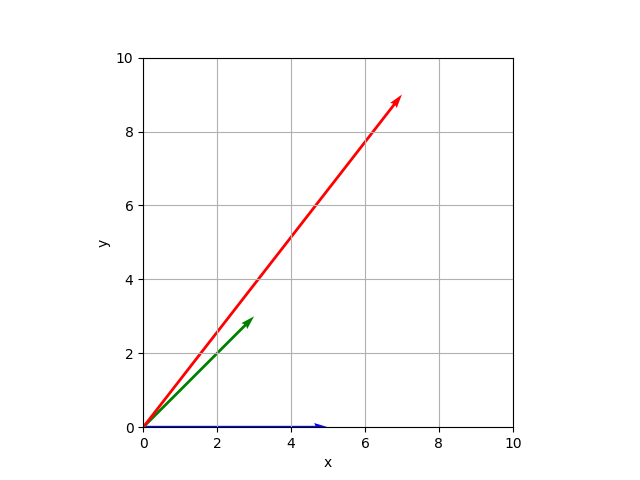
\includegraphics[width=0.4\textwidth]{Images/1/vectors.png}
    \hspace{2cm} 
    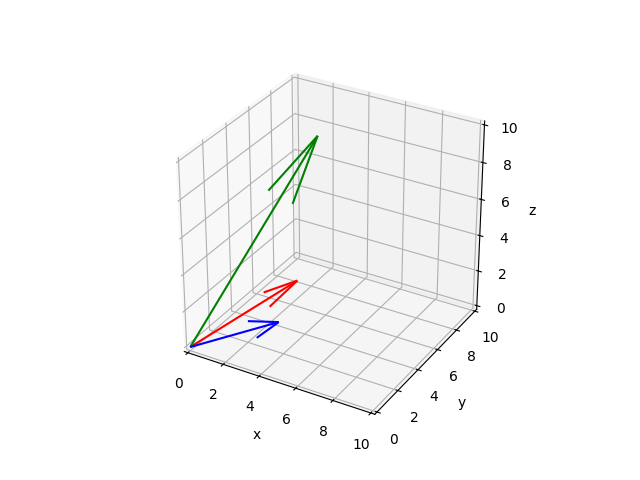
\includegraphics[width=0.4\textwidth]{Images/1/vectors_3d.png}
    \caption{Visualización de vectores en $\R^2$ y $\R^3$ respectivamente.}
    \label{fig:imagenes}
\end{figure}

\lipsum[1]

\subsection{Examples 2}
